\chapter{Partikelrörelse i celler}

Partikelrörelse i cellers cytoplasma är något som fortfarande förundrar forskare inom biofysik~\cite{Hofling&Franosch2013}. En enkel modell som modellerar partikelrörelserna som klassisk brownsk rörelse kan inte förklara de observerade egenskaperna. Där är en långsammare diffusion, subdiffusion, en av de tydligaste avvikelserna från brownsk rörelse. Andra modeller har tagits fram i avsikt att försöka förklara rörelsen men i dagsläget finns inte någon universell modell som kan beskriva rörelsen fullständigt. 
Detta kapitel presenterar inledningsvis tre möjliga förklaringsmodeller till partikelrörelsen:  Ornstein-Uhlenbeck-processen, CTRW och fBm.


I denna studie undersöks om given data över partikelrörelse i jästceller har egenskaper, bland annat MSD och asfärisitet, som kan beskrivas av dessa modeller. Både teoretiska beräkningar och simuleringar används för att göra jämförelsen. 

Av de olika modellerna är Ornstein-Uhlenbeck-processen den enklaste, men på grund av detta ärver den lite för många egenskaper från brownsk rörelse för att kunna förklara subdiffusionen. Härav kommer de mer komplicerade modellerna in -- CTRW och fBm.
Den största skillnaden mellan CTRW och fBm är att CTRW är en icke-stationär process medan stegen i fBm är stationära. Något som används för att avgöra deras relevans som förklaringsmodeller. 

Några av de viktigaste resultaten i detta kapitel är att rörelsen är subdiffusiv och verkar vara stationär.
Av detta dras slutsatsen att vanlig brownsk rörelse inte är tillräcklig för att förklara partikelrörelsen här, och att fBm är en mer trolig kandidat som förklaringsmodell än CTRW. Dock verkar ingen av modellerna ge helt tillfredsställande förutsägelser.
Vidare visar även studierna att rörelsen är minst lika isotrop som en vanlig brownsk rörelse. Det verkar alltså inte finnas några större anisotropier i cellerna som påverkar partikelrörelsen.



\subsubsection{Undersökt data}
Datan som studerats för partikelrörelse är samma som \cite{Midtveldt_etal2016} använde och utgörs av mätningar av positionen för fluorescerande partiklar i jästceller. Jästcellerna hade genmodifierats till att producera fluorescerande protein som lätt bildar kluster. Dessa kluster brukar vara av storleksordning 0,1--0,5\,\micro{m}, vilket kan jämföras med själva cellernas storlek på omkring 5\,\micro{m}.

Data för ett hundratal partiklar från olika jästceller ingick i mätserien, både för aktiva celler och celler som försatts i dvala, alltså celler med sänkt metabol aktivitet. Mätningen genomfördes med 100 bilder per sekund.



\section{Modeller för partikelrörelse i vätskor}

Till en första approximation skulle partikelrörelser i cytoplasman kunna beskrivas med klassisk brownsk rörelse. Detta är en enkel modell med en tydlig fysikalisk tolkning -- att många mindre molekyler krockar med partiklarna så att partiklarna börjar vandra runt. Den här modellen har dock en teoretisk svaghet i att den förutsätter att systemet är i termisk jämvikt~\cite{Einstein1905,Hofling&Franosch2013}, något som inte är fallet inuti levande celler. Vidare behöver cytoplasman inte nödvändigtvis gå att beskriva som en klassisk vätska\footnotemark{}~\cite{Midtveldt_etal2016}, som också krävs i Einsteins härledning~\cite{Einstein1905}.
\footnotetext{En klassisk vätska är en vätska som uppfyller Stokes lag för viskös friktion. }

Alltså finns redan vissa teoretiska invändningar mot att använda klassisk brownsk rörelse för att beskriva partikelrörelser med vanlig brownsk rörelse, men det slutgiltiga provet finns i experiment. 
Bland annat \cite{Parry_etal2014} och \cite{Midtveldt_etal2016} har visat att diffusionen av partiklar i celler är fundamentalt långsammare än förväntat från klassisk brownsk rörelse. 

För att visa detta används MSD, ett mått som mäter hur långt en partikel i medel förflyttar sig under en given tid. Som visades i avsnitt~\ref{sec:brown} är MSD:n för brownsk rörelse proportionell mot förlupen tid. Speciellt kan \eqref{eq:MSD_brown} skrivas om till
\begin{equation}
\ev{x(t)^2} \propto t,
\end{equation}
där $x(0)=0$. Vad man då har funnit i tidigare studier är att exponenten på $t$ är lägre än~$1$, vilket tyder på att andra modeller för partikelrörelserna kan behövas.


\subsection{Ornstein-Uhlenbeck-processen}
En första utvidgning av modellen för brownsk rörelse fås genom att lägga till en återförande term som drar partikeln mot någon medelpunkt. Detta är en så kallad Ornstein-Uhlenbeck-process
\begin{equation}\label{eq:SDE_o-u}
\pd_t x = -\gamma ( x-\bar{x} ) + \sigma\pd_t W,
\end{equation}
där $\gamma$ är en tidsskala som styr hur hårt bunden partikeln är till medelpositionen $\bar{x}$, och $\pd_t W$ är den stokastiska drivningen av partikeln som uppfyller \eqref{eq:white_noise}. 

Detta är en inte helt orimlig modell eftersom en partikel i en cell rimligtvis inte kan vandra hur långt som helst. Typiskt kommer en partikel att tränga ihop cytoplasmans beståndsdelar i den riktning som den rör sig åt, vilket leder till en återförande kraft.

Med \eqref{eq:SDE_o-u} och metoderna från avsnitt~\ref{sec:brown} kan modellens autokorrelation och MSD härledas. Autokorrelationen i gränsen mot ett stationärtillstånd ($\gamma t\gg 1$) blir då i en dimension
\begin{equation}\label{eq:COV_o-u}
\ev{x(t)x(t+\Delta{t})} \approx \frac{\sigma^2}{2\gamma} \ee^{-\gamma\Delta{t}},
\end{equation}
där $\bar{x}$ har satts till 0. Vidare kan också MSD beräknas; med $\Delta{t}=\abs{t-t'}$ erhålls
%Med \eqref{eq:SDE_o-u} och metoderna från avsnitt~\ref{sec:brown} kan bland annat modellens MSD beräknas. Med $\bar{x}=0$ blir MSD:n 
\begin{equation}\label{eq:MSD_o-u}
\ev{\Big(x(t)-x\big(t'\big) \Big)^2} 
\approx \frac{\sigma^2}{\gamma} \left( 1-\ee^{-\gamma \Delta{t}} \right).
\end{equation}
%där $\Delta{t}=\abs{t-t'}$. Approximationen ovan gäller i den stationära gränsen $t, t'\gg\nicefrac{1}{\gamma}$, när eventuella initialbeteenden har dött ut.



\subsection{Continuous Time Random Walk (CTRW)}
En möjlig förklaringsmodell för anomal transport i celler utgörs av CTRW (Continuous-Time Random Walk)~\cite{Hofling&Franosch2013}. Här beskrivs rörelsemönstret av att partiklarna under majoriteten av tiden sitter bundna till olika nätliknande strukturer för att sedan plötsligt ta sig vidare till en ny position efter en viss tid. Partiklarnas steglängder samt väntetider mellan steg är stokastiska variabler. För härledning av partikelns egenskaper givet en CTRW modell, se bilaga~\ref{app:CTRW}. 

Den stora skillnaden mellan en CTRW modell och enkel slumpvandring är att väntevärdet av tiden mellan två steg kan vara odefinierad för en CTRW modell. I dessa fall används ofta \cite{Hofling&Franosch2013} fördelningsfunktionen som för stora $t$ asymptotiskt går mot
\begin{equation}
\psi(t) \sim \frac{1}{t^{\alpha+1}}\qcomma 0<\alpha<1,
\end{equation}
där $\psi$ är sannolikhetstätheten för partikelns väntetid. Att fördelningen avtar som ett potenssamband gör att väntevärdet, enligt \eqref{eq:EV}, inte existerar för väntetiden.

Givet att väntevärdet av steglängden är noll så blir MSD för CTRW vid stora tider
\begin{equation}\label{eq:CTRW_MSD}
    \ev{x(t)^2} \propto t^{\alpha} \qcomma 0<\alpha<1.
\end{equation}
Eftersom $0<\alpha<1$ utför CTRW subdiffusion, som är vad som observerats. Denna anomala transport uppstår eftersom väntevärdet av tiden mellan steg är odefinierad, vilket medför att centrala gränsvärdessatsen ej uppfylls. Summan av de stokastiska variablerna går således ej mot att bli normalfördelad, något som är grundläggande för teorin kring brownsk rörelse.

CTRW är en icke-stationär process vilket medför att MSD:n i \eqref{eq:CTRW_MSD} beräknas från startpositionen $x(0)=0$. En beräkning av MSD mellan två andra tidpunkter skulle medföra ett explicit tidsberoende, det vill säga inte enbart bero på tidsskillnaden mellan tidpunkterna.

%\todo[color=lime]{kanske något om att subdiffusion uppstår då man medelvärderar över många partiklar}

\begin{comment}
Positionsändringen och väntetiden beskrivs av två oberoende stokastiska variabler. 
MSD för denna typ av rörelse blir\cite{Barkai_MSDCTRW2007}
\begin{equation}
    \ev{x^2(t)} \approx \frac{\ev{\Delta x^2}}{A \Gamma(1+\alpha)}t^{\alpha} + \frac{2\ev{\Delta x}^2}{\Gamma(1+2\alpha)A^2} t^{2\alpha}, 
\end{equation}
där $A$ är en konstant som dyker upp i fördelningsfunktionen för väntetiderna, $\Gamma$ är gammafunktionen, $\alpha$ en konstant som uppfyller $0<\alpha<1$ och $\Delta x$ steget mellan två positioner. Om $\ev{\Delta x}=0 $ försvinner andra termen och rörelsens MSD blir proportionell mot $t^\alpha$. Eftersom $\alpha < 1$ blir MSD:n inte linjär i tiden, utan ändringstakten kommer att avta med tiden och rörelsen skiljer sig från den klassiska brownska rörelsen.
\end{comment}

Den här modellen har visat sig kunna beskriva vissa aspekter av partikelrörelse i nät av F-aktinfilament\cite{Barkai_CTRW}. Om partikelns radie var av samma storleksordning som genomsnittliga maskstorleken bands partiklarna tillfälligt i nätet, bortsett från termiska fluktuationer, för att sedan ta sig igenom en maska och fastna i ett nytt hålrum i nätet. MSD:n för dessa partiklar uppfyllde ett $t^{\alpha}$-beroende som i \eqref{eq:CTRW_MSD}. Partiklar med radier som var betydligt mindre än maskstorleken hade ett rörelsemönster mer likt brownsk rörelse medan de större partiklarna fastnade i nätet utan att kunna ta sig loss.
%Om en liknande nätstruktur kan uppstå i jästceller kan man alltså förvänta sig olika resultat vad gäller rörelsen för partiklar av olika storlek.

%Lästips:
%https://faculty.biu.ac.il/~barkaie/PCCPreview.pdf
%https://faculty.biu.ac.il/~barkaie/Pathways.pdf


\subsection{Fractional Brownian Motion (fBm)}

En annan modell som undersöks är fractional Brownian motion~\cite{Mandelbrot_fBm1968} som bygger på superpositioner av Wienerprocesser med steg som uppvisar en nollskild korrelation i tiden. För en formell definition och härledning av nedanstående egenskaper hänvisas läsaren till bilaga~\ref{sec:App_fBm}.

En \emph{normerad} fBm $B_H(t)$ kan karakteriseras helt~\cite{Dieker_fBm} från att $B_H(t)$ har stationära och gaussiskt fördelade steg för varje tid $t$, $B_H(0)=0$ samt
\begin{equation}
\begin{aligned}
    \ev{B_H(t)}&=0 \\
    \ev{B^2_H(t)}&=\abs{t}^{2H}
\end{aligned}
\end{equation}
där Hurstparametern $H$ uppfyller $0< H <1$. För $H=\nicefrac{1}{2}$ återfås vanlig brownsk rörelse. 

Stationära förändringar medför att variansen för stegen mellan två tidpunkter $t_1$ och $t_2$ är
\begin{equation} \label{eq:fBm_MSD}
    \ev{(B_H(t_1)-B_H(t_2))^2} = \abs{t_1-t_2}^{2H};
\end{equation}
variansen saknar explicit tidsberoende och beror därmed bara på tidsintervallets storlek. 

Stegen mellan varje positionsändring i en normerad fBm:  $\delta(t)=B_H(t+T)-B_H(t)$ är standardnormalfördelad för varje tid $t$ men till skillnad från ren brownsk rörelse är stegen i allmänhet inte oberoende.

Kovariansen för fBm fås genom att utnyttja de karakteristiska egenskaperna till att bli
\begin{equation} %Ta ej bort kovariansen då hör samman med stycket nedan
\COV{B_H(t_1)}{B_H(t_2)}=\ev{B_H(t_1)B_H(t_2)}
= \frac{1}{2} 
\left(\abs{t_1}^{2H}+\abs{t_2}^{2H}-\abs{t_2-t_1}^{2H}\right).
\end{equation}
Detta ger att för $H>\nicefrac{1}{2}$ fås positiv korrelation mellan två positioner i rörelsen, och för $H<\nicefrac{1}{2}$ blir korrelationen negativ. Den negativa korrelationen ger ett ''hackigare'' utseende åt rörelsen då den ofta byter riktning. Den positiva korrelationen ger istället kurvan ett mer slätt utseende som tenderar att dra iväg i en bestämd riktning. Det förstnämnda fallet ger subdiffusion medan det andra fallet ger superdiffusion -- långsammare respektive snabbare diffusion än vanlig brownsk rörelse. 

Utöver den normerade fBm finns även en icke-normerad variant av rörelsen. Den stora skillnaden mellan de två är att variansen för stegen får en extra, konstant faktor.

Även om fBm har stationära steg är processen i sig inte stationär \cite{Flandrin_fBmspektrum1989}, vilket ger en tidsberoende spektraltäthet. Istället kan det vara av intresse att betrakta de stationära stegen, $\delta (t)$, för en fBm
\begin{equation}
    \delta(t)=B_H(t+T)-B_H(t)
\end{equation} 
kallade fractional Gaussian noise (fGn), där $T$ är tiden mellan två samplingar. PSD:n för dessa beräknas i bilaga~\ref{sec:App_fBm}. De blir i det icke-normerade fallet
\begin{equation}
    \mathcal{S}_{\hat{\delta}}(\omega)=4\left(\sin{\frac{\omega T}{2}}\right)^2 \abs{\omega}^{-(2H+1)}
\end{equation}
det vill säga oberoende av tiden $t$, där $\hat{\delta}$ är fGn för en icke normerad fBm. Här representerar $\omega$ vinkelfrekvensen.

Mätningar~\cite{Mandelbrot_fBm1968} på diffusionsartade stokastiska processer har visat på starkt beroende även mellan steg som är separerade långt i tid. Detta kan inte förklaras med den brownska rörelsens okorrelerade steg, vilket motiverar införandet av denna modell som kandidat för att beskriva diffusion i celler. 


\section{Intensitets- och storleksberoende samt brusundersökning} \label{sec:storleksberoende}
%Om värdena skiljer sig åt väsentligt för små och stora partiklar -> CTRW mer trolig. 

Den studerade datan består av ett hundratal olika partiklar i respektive fas. Alla dessa partiklarna har olika storlek, vilket speglas i att de får olika hög intensitet när de filmas genom ett mikroskop. I nuläget finns ingen bra kännedom om hur en partikels intensitet förhåller sig till dess radie. I \cite{Parry_etal2014}, som hade samma sorts partiklar som här, gjordes ett försök att jämföra med partiklar med känd storlek. De lyckades dock inte säkert fastställa något tydligt samband.

Den här studien kommer inte att försöka reda ut något samband mellan en partikels intensitet och storlek. Men för att kunna ta medelvärden som inte påverkas av partikelstorlek behövs ändå vissa samband mellan dess intensitet och hur mycket partikeln rör sig.

För det första behövs en definition på ''hur mycket partikeln rör sig''. En sådan definition bör spegla den egenskap som man vill undersöka via medelvärdering. I de flesta fall, exempelvis MSD, visar sig positionens varians vara ett lämpligt mått att använda för normering. Dock används inte variansen som direkt normering eftersom det egentligen är \emph{intensiteten} som ska korrigeras för.

Ett samband behöver alltså anpassas mellan intensitet $I$ och positionens varians
\begin{equation}
\sigma_r^2=\sigma_x^2+\sigma_y^2,
\end{equation}
som alltså ges av summan av varianserna i $x$- och $y$-led.
Ett av de enklaste sambanden att ansätta är ett potenssamband:
\begin{equation}
\sigma_r^2 \propto I^{\tilde\beta} 
\Longleftrightarrow 
\sigma_r \propto I^\beta.
\end{equation}
Ett sådant samband svarar mot en trendlinje i en dubbellogplott, där $\beta$ blir linjens lutning. I efterföljande undersökningar kan sedan denna trendlinje användas för att vikta termer från olika partiklar i medelvärden. % så att intensitetsvariationerna korrigeras.

\subsubsection{Undersökning av mätbrus}
En viktig aspekt i alla fysikaliska mätningar är hur mycket brus datan innehåller. Så även i den här studien. Dock kan det verka motsägelsefullt att försöka uppskatta hur mycket brus man har i data som består av slumpvandrande partiklar -- också det ett sorts ''brus''. Det går dock att göra några försök. 

Mätbruset kan uppskattas genom att ansätta en uppmätt position på formen
\begin{equation}
\hat{x}_i = x_i(I) + \sigma_\text{brus}\eta_i,
\end{equation}
där $x_i(I)$ är den verkliga positionen och $\sigma_\text{brus}\eta_i$ är ett oberoende normalfördelat mätbrus med standardavvikelse $\sigma_\text{brus}$. Vidare antas även att partiklarnas verkliga rörelse minskar med ökad storlek så att mätbruset blir dominant hos partiklar med stora intensiteter:
\begin{equation}\label{eq:approx_noise}
\hat{x}_i \approx \sigma_\text{brus}\eta_i \qcomma \text{för stora } I.
\end{equation}
Med detta går det nu att uppskatta mätbrusets styrka, $\sigma_\text{brus}$, genom att undersöka exempelvis steglängdens asymptotiska beteende. 

Om man undersöker medelsteglängden $\Delta{\bar{r}}$ under antagandet att \eqref{eq:approx_noise} gäller finner man att
\begin{equation}\label{eq:delta_r_noise}
\begin{aligned}
\Delta{\bar{r}} =& 
\ev{\sqrt{ (\hat{x}_{i+1}-\hat{x}_{i})^2 + (\hat{y}_{i+1}-\hat{y}_{i})^2 } }_{\!i}
\\
\approx& 
\sigma_\text{brus} \ev{ \sqrt{ \left(\eta^{(x)}_{i+1} - \eta^{(x)}_{i}\right)^2 + \left(\eta^{(y)}_{i+1}-\eta^{(y)}_{i}\right)^2} }_{\!i} 
\\
=&\sqrt{\pi} \sigma_\text{brus}.
\end{aligned}
\end{equation}
Här användes att väntevärdet för en $\chi_k$-fördelning ges av
$\sqrt{2}\,\Gamma(\nicefrac{k+1}{2})/\Gamma(\nicefrac{k}{2})$ \cite{wiki:chi-distribution}
för att evaluera den andra raden i \eqref{eq:delta_r_noise}.\footnotemark{}
\footnotetext{Mer specifikt användes att $(\eta_{i+1}-\eta_i)\sim N(0,\sqrt{2})$, vilket ger att \cite{wiki:chi-distribution}
\[ 
\sqrt{ 
 \left( \nicefrac{\left( \eta^{(x)}_{i+1}-\eta^{(x)}_{i} \right)}{\sqrt{2}} \right)^2 
+\left( \nicefrac{\left( \eta^{(y)}_{i+1}-\eta^{(y)}_{i} \right)}{\sqrt{2}} \right)^2
} 
\sim \chi_2.
\]
Härav följer att väntevärdet på mittenraden i \eqref{eq:delta_r_noise} blir 
$\sqrt{2} 
\left(\sqrt{2}\Gamma(3/2)/\Gamma(1)\right) 
= 2\Gamma(\nicefrac{3}{2})=\sqrt{\pi}.$
}

Med samma antagande, \eqref{eq:approx_noise}, kan även partikelns standardavvikelse användas för brusuppskattning. I gränsen med stora $I$ blir
\begin{equation}\label{eq:sigma_r_noise}
\begin{aligned}
\sigma_r =& 
\sqrt{\VAR{\hat{x}_i} + \VAR{\hat{y}_{i}} }\\
%\approx& \sigma_\text{brus} \sqrt{\VAR{\eta^{(x)}} + \VAR{\eta^{(y)}} }\\
\approx&\sqrt{2}\,\sigma_\text{brus}.
\end{aligned}
\end{equation}
Fast här användes istället att $\VAR{\eta^{(x)}} = \VAR{\eta^{(y)}} =1$.


\subsection{Resultat -- olika starkt intensitetsberoende mellan de olika cellfaserna} \label{sec:resultat-storleksberoende}

\begin{figure}\centerline{
   \subfigure[][]{\input{bilder/partiklar/std_ed.tex}}
   \subfigure[][]{\input{bilder/partiklar/std_lp.tex}}
   }\centerline{
   \subfigure[][]{\input{bilder/partiklar/medelsteg_ed.tex}}
   \subfigure[][]{\input{bilder/partiklar/medelsteg_lp.tex}}
   }
\caption{Varje enskild partikels standardavvikelse $\sigma_r$ och medelsteglängd $\Delta{\bar{r}}$ plottade mot deras intensitet $I$ i mikroskopet. 
Med standardavvikelse menas hur stor standardavvikelse partikeln hade i sin position enligt $\sigma_r=(\sigma_x^2+\sigma_y^2)^{1/2}$, där $\sigma_x$ och $\sigma_y$ är standardavvikelserna i $x$- respektive $y$-koordinaten.
%En partikels intensitet svarar mot dess storlek, så det vore rimligt att deras steglängder och standardavvikelse asymptotiskt går mot $0$.
Från steglängdens asymptotiska beteende för stora intensiteter uppskattades mätbrusets storlek. 
Anledningen till att brusnivån skiljer sig åt mellan medelsteg och standardavvikelse är att det kommer in olika faktorer för ett mätbrus i de olika måtten -- se \eqref{eq:delta_r_noise} och \eqref{eq:sigma_r_noise}. 
Här visas också vad en brusnivå på 11\,nm skulle motsvara; detta görs för att \cite{Midtveldt_etal2016}, som använde samma data, kom fram till att bakgrundsbruset var så stort.}
\label{fig:storleksberoende}
\end{figure}

De trendlinjer som har anpassats till $\sigma_r$ är gjorda som potenssamband; på så sätt erhålls \emph{linjer} i en dubbellogplott. Anpassningarna visas i \figref{fig:storleksberoende}. Det verkar finnas någon trend i $\sigma_r$, men den är inte helt tydlig. 
Det finns dock en viss skillnad mellan celler i dvala och i log-fas med avseende på hur intensitetsberoendet ser ut. Vidare verkar det finnas en mycket tydligare trend i medelstegen, men eftersom det framförallt är $\sigma_r$ som används som viktning så togs trendlinjer fram för $\sigma_r$ istället.

%Brus
Eftersom \eqref{eq:delta_r_noise} har en något större faktor framför $\sigma_\text{brus}$ används $\Delta{\bar{r}}$ för att bestämma $\sigma_\text{brus}$ -- i \figref{fig:storleksberoende} syns också att det finns ett tydligare trendbrott i medelsteglängderna än i standardavvikelserna. Det bestämda värdet på brusnivån, $\sigma_\text{brus}$, från $\Delta{\bar{r}}$ kan sedan användas i \eqref{eq:sigma_r_noise} för att se om $\sigma_r$ ser ut att gå mot det beräknade värdet $\sqrt{2}\sigma_\text{brus}$. Detta borde i så fall synas i form av en avvikelse från trendlinjen där den korsar brusnivån.
I fallet med celler i dvala, \figref{fig:storleksberoende}~(a) och (c), ser det ut att kunna stämma, men data saknas tyvärr i just det intressanta området. Partiklarna från celler i log-fasen, \figref{fig:storleksberoende}~(b) och (d), har ett mycket svagare intensitetsberoende och där går det inte att säga något om huruvida den beräknade brusnivån stämmer. 

Egentligen är den enda indikationen på att det skulle finnas en brusnivå utplaningen\footnotemark{} i \figref{fig:storleksberoende}~(c). Och om det rör sig om mätbrus borde $\sigma_\text{brus}$ vara samma för partiklar i båda cellerfaserna eftersom datan var insamlad på samma sätt och med samma utrustning. Sammantaget ger denna brusanalys alltså att mätbrusets storlek bör väljas från celler i dvala. Brusnivån blir då $\sigma_\text{brus}=\unit[5]{nm} \pm 10\,\%$. Här har osäkerheten beräknas genom att ta standardavvikelsen i $\Delta\bar{r}$ för de partiklar vars intensitet översteg $16$\,intensitetsenheter i \figref{fig:storleksberoende}.

\footnotetext{Läsaren påminns om att $I$-axeln är logaritmerad, vilket leder till att området från 5--20 ser betydligt mindre ut i jämförelse med hela intervallet än vad det är. Detta gör tyvärr att utplaningen inte ser ut att vara så betydelsefull. }




\section{Undersökning av olika typer av MSD}

I det här avsnittet jämförs data med de tidigare nämnda modellernas förutsägelser. Bland annat räknades det fram i avsnitt~\ref{sec:brown} att MSD:n för en sådan partikel skulle öka linjärt med tiden, se \eqref{eq:MSD_brown}.

Vidare finns det minst två sätt att beräkna partiklarnas MSD. För stationära processer, det vill säga processer som inte explicit beror på när i tiden de inleds, kan man skapa ett medelvärde mellan alla möjliga mätpunkter separerade med givet tidsintervall $\Delta{t}$ enligt
\begin{equation} \label{eq:MSD_S}
S(\Delta t)= \frac{1}{N}\sum^N_{i=1}\frac{1}{m}\sum^m_{j=1}
\Big( x_i(t_j+\Delta t)-x_i(t_j) \Big)^2,
\end{equation} 
där $N$ är antalet partiklar och $m$ antalet möjliga tidsintervall av längd $\Delta t$. 
Man kan också betrakta
\begin{equation} \label{eq:MSD_s}%Byta plats?
s(\Delta t)= \frac{1}{N}\sum^N_{i=1}
\Big( x_i(\Delta t)-x_i(0)\Big )^2,
\end{equation} 
som inte kräver att processen är stationär.
Genom att jämföra resultatet mellan dessa två typer av MSD kan man avgöra om processen är stationär. Detta eftersom en stationär process är oberoende av tidstranslation och därmed borde ge samma resultat för $S$~och~$s$. 

De givna ekvationerna gäller för ändliga och diskreta datamängder, men $S$~och~$s$ skulle också kunna beskrivas teoretiskt med en väntevärdesbeskrivning.

En annan skillnad som kan uppstå när man beräknar MSD med \eqref{eq:MSD_S} respektive \eqref{eq:MSD_s} är att i en praktisk tillämpning, med begränsad datamängd, så kan $S(\Delta{t})$ bli betydligt jämnare än $s(\Delta{t})$. Detta på grund av att \eqref{eq:MSD_S} innehåller betydligt fler termer i varje medelvärde. 



\subsection{Resultat -- ingen märkbar skillnad mellan olika MSD-mått}


För att undersöka om partikelrörelsen utgör en stationär process beräknas de olika MSD måtten för partiklarna enligt \eqref{eq:MSD_S} och \eqref{eq:MSD_s}. Ett potenssamband har anpassats till resultaten i de båda beräkningarna och visas i \figref{fig:MSD}. 

Ingen väsentlig skillnad i exponenten kan uttydas från anpassningen mellan de två MSD-typerna. Detta tyder på att processen är stationär. Partikelrörelserna torde därför inom detta område kunna beskrivas bättre av den stationära fBm snarare än den icke-stationära CTRW.

Jämförs exponenterna i potensanpassningen mellan cellerna i dvala och log-fas, (a) respektive (b) i \figref{fig:MSD}, finns en viss skillnad. Exponenten för cellerna i dvala är $0,60$ mot log-fas-cellernas $0,80$. Med osäkerhetsgränser som i \figref{fig:MSD_error} syns att dessa värden på exponenterna själva får en osäkerhet på ungeför $\pm 0,05$. Även om \figref{fig:MSD_error} bara visar detta för partiklar från celler i dvala så gäller samma osäkerhet i exponenten för celler i log-fas.

Även med felgränserna för exponenterna syns dock att båda processerna ändå är exempel på subdiffusion. Alltså att partiklarnas MSD beror av tiden som ett potenssamband med exponent mindre än $1$. Subdiffusion är en avvikelse från klassisk brownsk rörelse, där exponenten enligt \eqref{eq:MSD_brown} ska vara $1$. 


Vidare ser $S$ och $s$ ut att ha ungefär samma värde för samma $\Delta{t}$. Detta beror på normeringen från avsnitt~\ref{sec:storleksberoende} som använts för att normera mot intensiteten. Men då det bara är lutningen, i dubbellogplot, på MSD:n som är intressant så påverkas inte resultaten av vilka absoluta värden MSD:n har.


\newgeometry{top=3cm, bottom=4cm} %Den här används för att få plats med båda figurerna på samma sida.
\begin{figure}\centerline{
\subfigure[][]{\input{bilder/partiklar/MSD_ed.tex}}
\subfigure[][]{\input{bilder/partiklar/MSD_lp.tex}}
}
\caption{Dubbellogplott av de olika sorternas MSD, beräknade enligt \eqref{eq:MSD_S} respektive \eqref{eq:MSD_s}, för de olika cellfaserna, dvala (a) och log-fas (b). På grund av normeringen som användes kommer $S(\Delta{t})$ och $s(\Delta{t})$ att ha samma värde i $\Delta{t}=\unit[10]{s}$. Detta är dock av liten betydelse eftersom det intressanta är lutningen i dessa grafer. I de olika cellfaserna syns att lutningarna i diagrammen är samma inom varje cellfas, men skiljer sig åt mellan (a) och (b). Detta tyder på ett stationärt beteende, men att det ändå finns en tydlig skillnad mellan aktiva celler och de i dvala. %Notera också att $S$ är jämnare än $s$, vilket bara beror på att $S$ innehåller fler termer som medelvärderats. 
}
\label{fig:MSD}
\end{figure}
\begin{figure}\centerline{
\subfigure[][]{
\input{bilder/partiklar/MSD_error_S.tex}
}
\subfigure[][]{
% GNUPLOT: LaTeX picture with Postscript
\begingroup
  \makeatletter
  \providecommand\color[2][]{%
    \GenericError{(gnuplot) \space\space\space\@spaces}{%
      Package color not loaded in conjunction with
      terminal option `colourtext'%
    }{See the gnuplot documentation for explanation.%
    }{Either use 'blacktext' in gnuplot or load the package
      color.sty in LaTeX.}%
    \renewcommand\color[2][]{}%
  }%
  \providecommand\includegraphics[2][]{%
    \GenericError{(gnuplot) \space\space\space\@spaces}{%
      Package graphicx or graphics not loaded%
    }{See the gnuplot documentation for explanation.%
    }{The gnuplot epslatex terminal needs graphicx.sty or graphics.sty.}%
    \renewcommand\includegraphics[2][]{}%
  }%
  \providecommand\rotatebox[2]{#2}%
  \@ifundefined{ifGPcolor}{%
    \newif\ifGPcolor
    \GPcolortrue
  }{}%
  \@ifundefined{ifGPblacktext}{%
    \newif\ifGPblacktext
    \GPblacktexttrue
  }{}%
  % define a \g@addto@macro without @ in the name:
  \let\gplgaddtomacro\g@addto@macro
  % define empty templates for all commands taking text:
  \gdef\gplbacktext{}%
  \gdef\gplfronttext{}%
  \makeatother
  \ifGPblacktext
    % no textcolor at all
    \def\colorrgb#1{}%
    \def\colorgray#1{}%
  \else
    % gray or color?
    \ifGPcolor
      \def\colorrgb#1{\color[rgb]{#1}}%
      \def\colorgray#1{\color[gray]{#1}}%
      \expandafter\def\csname LTw\endcsname{\color{white}}%
      \expandafter\def\csname LTb\endcsname{\color{black}}%
      \expandafter\def\csname LTa\endcsname{\color{black}}%
      \expandafter\def\csname LT0\endcsname{\color[rgb]{1,0,0}}%
      \expandafter\def\csname LT1\endcsname{\color[rgb]{0,1,0}}%
      \expandafter\def\csname LT2\endcsname{\color[rgb]{0,0,1}}%
      \expandafter\def\csname LT3\endcsname{\color[rgb]{1,0,1}}%
      \expandafter\def\csname LT4\endcsname{\color[rgb]{0,1,1}}%
      \expandafter\def\csname LT5\endcsname{\color[rgb]{1,1,0}}%
      \expandafter\def\csname LT6\endcsname{\color[rgb]{0,0,0}}%
      \expandafter\def\csname LT7\endcsname{\color[rgb]{1,0.3,0}}%
      \expandafter\def\csname LT8\endcsname{\color[rgb]{0.5,0.5,0.5}}%
    \else
      % gray
      \def\colorrgb#1{\color{black}}%
      \def\colorgray#1{\color[gray]{#1}}%
      \expandafter\def\csname LTw\endcsname{\color{white}}%
      \expandafter\def\csname LTb\endcsname{\color{black}}%
      \expandafter\def\csname LTa\endcsname{\color{black}}%
      \expandafter\def\csname LT0\endcsname{\color{black}}%
      \expandafter\def\csname LT1\endcsname{\color{black}}%
      \expandafter\def\csname LT2\endcsname{\color{black}}%
      \expandafter\def\csname LT3\endcsname{\color{black}}%
      \expandafter\def\csname LT4\endcsname{\color{black}}%
      \expandafter\def\csname LT5\endcsname{\color{black}}%
      \expandafter\def\csname LT6\endcsname{\color{black}}%
      \expandafter\def\csname LT7\endcsname{\color{black}}%
      \expandafter\def\csname LT8\endcsname{\color{black}}%
    \fi
  \fi
  \setlength{\unitlength}{0.0500bp}%
  \begin{picture}(4250.00,3968.00)%
    \gplgaddtomacro\gplbacktext{%
      \csname LTb\endcsname%
      \put(860,1093){\makebox(0,0)[r]{\strut{}$10^{-1}$}}%
      \csname LTb\endcsname%
      \put(860,1960){\makebox(0,0)[r]{\strut{}$10^{0}$}}%
      \csname LTb\endcsname%
      \put(860,2827){\makebox(0,0)[r]{\strut{}$10^{1}$}}%
      \csname LTb\endcsname%
      \put(980,440){\makebox(0,0){\strut{} 0,01}}%
      \csname LTb\endcsname%
      \put(1950,440){\makebox(0,0){\strut{} 0,1}}%
      \csname LTb\endcsname%
      \put(2919,440){\makebox(0,0){\strut{} 1}}%
      \csname LTb\endcsname%
      \put(3889,440){\makebox(0,0){\strut{} 10}}%
      \put(160,1733){\rotatebox{-270}{\makebox(0,0){\strut{}MSD /[godt. längdenhet$^2$]}}}%
      \put(2434,140){\makebox(0,0){\strut{}$\Delta{t}$ /[s]}}%
    }%
    \gplgaddtomacro\gplfronttext{%
      \csname LTb\endcsname%
      \put(3183,3755){\makebox(0,0)[r]{\strut{}\footnotesize $s(\Delta{t})$, dvala}}%
      \csname LTb\endcsname%
      \put(3183,3555){\makebox(0,0)[r]{\strut{}\footnotesize 95\,\% konfidensintervall}}%
      \csname LTb\endcsname%
      \put(3183,3355){\makebox(0,0)[r]{\strut{}\footnotesize Anpassning $\propto(\Delta{t})^{0,6\phantom{5}}$}}%
      \csname LTb\endcsname%
      \put(3183,3155){\makebox(0,0)[r]{\strut{}\footnotesize Ändrad exponent $\pm 0,05$}}%
    }%
    \gplbacktext
    \put(0,0){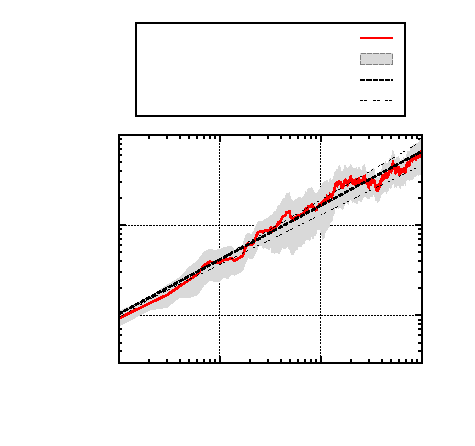
\includegraphics{MSD_error_s}}%
    \gplfronttext
  \end{picture}%
\endgroup

}}
\caption{Dubbellogplott av de olika sorternas MSD för celler i dvala med felgränser och möjliga anpassningar. De olika MSD:erna beräknades med \eqref{eq:MSD_S} respektive \eqref{eq:MSD_s}. Felgränserna är satta som konfidensintervall med 95\,\% konfidens. Med felgränserna syns att exponenten kan variera omkring $\pm 0,05$; detta visar sig också vara fallet för celler i log-fas.}
\label{fig:MSD_error}
\end{figure}
\restoregeometry%återställer inställningarna till det normala




\section{Isotropi i partikelrörelsen} \label{sec:isotropi}
Om man misstänker att cellens inre struktur påverkar partikelrörelserna skulle eventuell anisotropi kunna ge ett bidrag till dessa. Alltså ifall det finns föredragna riktningar för partikeln att röra sig i. Ett sätt att undersöka detta är genom att betrakta koordinaternas kovariansmatris
\begin{equation}\label{eq:C_matris}
\mathsf{C}=
\begin{bmatrix} 
\ev{x^2}-\ev{x}^2 & \ev{xy}-\ev{x}\ev{y}\\
\ev{yx}-\ev{x}\ev{y} & \ev{y^2}-\ev{y}^2
\end{bmatrix}.
\end{equation}

Notera hur snarlik $\mathsf{C}$ är tröghetsmatrisen för en kropps olika tröghetsmoment, som uppkommer i mekaniken. Och precis som i mekaniken kan man hitta två principalaxlar genom att ta fram dess egenvektorer och diagonalisera matrisen. I mekaniken svarar principalaxlarna mot de riktningar där rörelsemängdsmomentet är oberoende av rotation längs andra axlar. I de här statistiska sammanhangen finns det en liknande tolkning, nämligen att principalaxlarna svarar mot de riktningar i cellen där rörelserna är oberoende av varandra. Egenvärdena i dessa två riktningarna svarar mot variansen i den oberoende koordinaten längs med den riktningen. 

Det går dessutom att visa att  egenvektorerna till $\mathsf{C}$ pekar i de riktningar i rummet med \emph{störst} respektive \emph{minst} varians \cite{Shlens_PCA2014}. Således kommer de två egenvektorerna, i de här fallen, att peka längs riktningen med störst respektive minst varians. Egenvärdena ger ett mått på hur bred fördelningen är i respektive riktning.


För att ur denna informationen få ut ett mått på hur isotropt partikeln rör sig kan man undersöka asfärisiteten~\cite{Rudnick_Asphericity1986}
\begin{equation}\label{eq:asph._2D}
    A=\frac{\ev{(\lambda_1 - \lambda_2)^2}}{\ev{(\lambda_1 + \lambda_2)^2}},
\end{equation}
som består av egenvärdena $\lambda_i$ till $\mathsf{C}$.
Om positionerna är helt isotropt fördelade så blir $\lambda_1=\lambda_2$, vilket ger $A=0$; om partikeln bara rör sig längs en linje blir istället $A=1$.

Det går även att generalisera \eqref{eq:asph._2D} till $d$ dimensioner:
\begin{equation}\label{eq:asph.}
    A_d=\frac{\sum_{j=1}^d\sum_{i<j} 
\ev{(\lambda_i-\lambda_j)^2} }{
(d-1) \ev{(\sum_{j=1}^d \lambda_j)^2}},
\end{equation}
som kan användas för mer avancerade teoretiska studier.


\subsubsection{Tillämpning av asfärisiteten}
Man kan enkelt visa att egenvärdena till kovariansmatrisen i \eqref{eq:C_matris} uppfyller~\cite{Hong_asymmetri1998}
\begin{equation}
\begin{aligned}
\lambda_1+\lambda_2 
&= \ev{x^2}-\ev{x}^2+\ev{y^2}-\ev{y}^2 
\\
\abs{\lambda_1-\lambda_2} 
&=\sqrt{\left(
            \left(\ev{x^2}-\ev{x}^2\right)^2
            -\left(\ev{y^2}-\ev{y}\right)^2
        \right)^2 
        +4(\ev{xy}-\ev{x}\ev{y})^2
}.
\end{aligned}
\end{equation}
För en given fördelningsfunktion med ändliga moment blir det därmed nu möjligt att beräkna denna kvot teoretiskt.

För en obegränsad Wienerprocess i $d$ dimensioner fås~\cite{Rudnick_Asphericity1986}
\begin{equation} \label{eq:Asphericity_Brownian}
    A_d^\text{(Wiener)}=\frac{2(d+2)}{5d+4}.
\end{equation}
I två dimensioner blir alltså $A_2^\text{(Wiener)}=\nicefrac{4}{7}$. Detta innebär att även oändligt långa brownska rörelser i snitt kommer att uppvisa viss asymmetri.

För fBm fås en formel i två dimensioner som gäller i gränsen där antalet mätpunkter blir mycket stort ~\cite{Hong_asymmetri1998}
\begin{equation} \label{eq:A_fBm}
A=2-
\frac{\frac{1}{2(H+1)^2}}{\frac{1}{2(H+1)^2}+\frac{2H+1}{4(4H+1)}-\frac{1}{4H+3}-\frac{\Gamma^2(2H+2)}{\Gamma(4H+4)}},
\end{equation}
där $H$ är Hurstparametern som karakteriserar rörelsen och $\Gamma$ är gammafunktionen. 

Med $H=\nicefrac{1}{2}$ fås vanlig brownsk rörelse, och asfärisiteten övergår till $A=\nicefrac{4}{7}$, vilket stämmer överens med ekvation \eqref{eq:Asphericity_Brownian} för $d=2$. Samma värde fås även approximativt för CTRW\cite{Ernst_ACTRW2012}.% eftersom denna rörelse vid varje tidsögonblick ser ut som brownsk rörelse. \todo[color=lime]{Kanske kan förklaras bättre?}

%Även http://iopscience.iop.org/article/10.1088/0305-4470/19/4/004/pdf



 
\subsection{Simulering och numerisk beräkning av asymmetrimått} 
\label{sec:sim_asym}
Istället för att bara direkt beräkna $A$ enligt \eqref{eq:asph._2D} kan man också studera fördelningen av måttet 
\begin{equation}\label{eq:asym}
\mathcal{A} =
\frac{(\lambda_1 - \lambda_2)^2}{(\lambda_1 + \lambda_2)^2}.
\end{equation}
Här ska det dock påpekas att i regel så är $A\neq\ev{\mathcal{A}}$ eftersom \eqref{eq:asph._2D} består av väntevärden i \emph{både} täljare och nämnare. Eftersom $\mathcal{A}$ alltså skiljer sig så från $A$ går det heller inte lika enkelt att göra teoretiska beräkningar, vilket gör att fördelningen av $\mathcal{A}$ får undersökas med Monte Carlo-simuleringar.


De modeller som testats är en vanlig Wienerprocess, en Wienerprocess med ett ''mätbrus'' pålagt och en Ornstein-Uhlenbeck-process. Tyvärr simulerades inte fBm och CTRW då dessa modeller är betydligt mer komplexa och behöver mer avancerade simuleringsalgoritmer. 
%Från dessa processer samt från datan över partikelrörelsen erhölls olika värden på $A$ och fördelningar av $\mathcal{A}$. 


För Wienerprocessen simulerades partikelns position i varje ny tidpunkt genom att gå ett normalfördelat steg från positionen i den förra tidpunkten. Detta kan skrivas som
\begin{equation}\label{eq:sim_wiener}
x_{i+1} = x_i + \sigma_\text{steg}\delta 
\qcomma  \delta \sim N(0, 1)
\end{equation}
och där $x_1=0$. Sedan gör man samma sak för $y$. Eftersom $\mathcal{A}$ ger ett mått på hur mycket partikeln \emph{föredrar en viss riktning} finner man att värdet på $\sigma_\text{steg}$ inte påverkar fördelningen -- så länge $\sigma_\text{steg}$ är samma för både $x$ och $y$. Detta blir uppenbart när man tänker på att \eqref{eq:sim_wiener} kan skrivas som 
$x_{i+1} =\sigma_\text{steg}\,x'_{i+1} = \sigma_\text{steg}\left( x'_i + \delta \right)$. 
Alltså att $\sigma_\text{steg}$ bara är en multiplikativ konstant framför positionen.

För att istället simulera en Wienerprocess med mätbrus användes \eqref{eq:sim_wiener} för att först simulera själva Wienerprocessen för att sedan \emph{efteråt} addera en slumpad brusterm $\sigma_\text{brus}\eta$ till varje position $x_i$. %Positionerna i simuleringen med brus ges alltså av
%\begin{equation}
%\hat{x}_{i} = x_i + \sigma_\text{brus}\eta 
%\qcomma  \eta \sim N(0, 1).
%\end{equation}
Den väsentliga skillnaden mot en ren Wienerprocess är att mätbruset $\eta$ inte påverkar nästkommande position. Till skillnad från den rena Wienerprocessen så kommer dock värdena på $\sigma_\text{steg}$ och $\sigma_\text{brus}$ att påverka $\mathcal{A}$, men enligt ett liknande argument som ovan kommer bara kvoten $\nicefrac{\sigma_\text{brus}}{\sigma_\text{steg}}$ vara det som påverkar. Detta gör att simuleringarna med mätbrus går att genomföra med olika värden på parametern $\nicefrac{\sigma_\text{brus}}{\sigma_\text{steg}}$ för att få olika fördelningar av~$\mathcal{A}$. 

Ornstein-Uhlenbeck-processen i \eqref{eq:SDE_o-u} simulerades genom att använda derivatan för tidsutveckling och genom att sätta $\bar{x}=0$. Man får då
\begin{equation}
x_{i+1} = x_i + \Delta{t}\,\pd_{t}x  = (1-k) x_i +  \sigma_\text{steg}\delta 
\qcomma  \delta \sim N(0, 1),
\end{equation}
där $x_1=0$. Notera här att den styrande parametern i simuleringarna är $k=\gamma\Delta{t}$, samt att $\sigma_\text{steg}$ på samma sätt som för den rena Wienerprocessen kan väljas godtyckligt utan att påverka $\mathcal{A}$. 

Samtliga simuleringar har gjorts med 1000 steg och 100\,000 upprepningar. Antalet steg valdes för att simuleringarna ska efterlikna den studerade datan -- som består av 1000 sparade positioner för varje partikel. Däremot kan upprepningarna väljas godtyckligt. Då valdes 100\,000 för ge tillräckligt jämna fördelningar.

%Vill Emelie lägga in något resultat om detta så får hon gärna lägga tillbaks det här stycket
%Eftersom resultatet för asymmetrimåttet i ekvation \eqref{eq:A_fBm} gäller för riktigt långa mätningar medan den data som analyseras i detta arbete är ganska begränsad kan man försöka simulera fram sannolikheter istället. Genom att simulera många mätserier för samma antal steg och antal partiklar som i datan kan man bedöma sannolikheten att det framräknade asymmetrimåttet till exempel skulle ha kommit från en ren klassisk brownsk rörelse. 


\subsection{Resultat -- partikelrörelserna är isotropa och behöver inte delas upp i anpassade koordinater}
\label{sec:resultat-isotropi}



Som kan ses i \figref{fig:asymmetri} skiljer sig den simulerade asfärisiteten $\mathcal{A}$ mellan partiklar från celler i dvala och de i log-fas. Båda fallen har fördelningar som svarar mot en rörelse som är minst lika isotrop som Wienerprocessen -- under de undersökta tidsskalorna. Vidare ses att partiklarna från celler i dvala får en fördelning av $\mathcal{A}$ med betydligt lägre sannolikhet för högre $\mathcal{A}$-värden, svarande mot mer asymmetriska rörelser. Skillnaden mellan cellfaserna tyder på att något förändras i cytoplasman när cellen går i dvala, något som påverkar partikelrörelserna. 

Om istället det riktiga asfärisitetsmåttet, $A$ från \eqref{eq:asph._2D}, betraktas erhålls värdena i \tabref{tab:asph._values} där uppmätta, teoretiska och simulerade värden presenteras med felgränser. %Det bör dock nämnas att det teoretiska värdet gäller i gräns mot när antalet steg går mot oändligheten medan de simulerade och uppmätta värdena beräknats från diskreta datamängder. Viss avvikelse kan därför vara att vänta. 
Från tabellen ses att de uppmätta värdena på $A$ blev $0,41\pm0,23$ för log-fas och $0,49\pm0,15$ för cellerna i dvala. På grund av de stora osäkerheterna kan dock inga säkra slutsatser dras.



\begin{figure}\centering
\input{bilder/partiklar/isotropi_asymmetri.tex}
\caption{Fördelning av asymmetrimåttet $\mathcal{A}$ enligt \eqref{eq:asym}, visat som sannolikheten att $\mathcal{A}$ är \emph{större} än ett visst värde $a$.
Graferna visar att de partiklar från celler i log-fas beter sig som en Wienerprocess. Partiklarna från celler i dvala beter sig däremot mer isotropt än en vanlig Wienerprocess; deras beteende skulle kunna modelleras som en Wienerprocess med pålagt brus med $\nicefrac{\sigma_\text{brus}}{\sigma_\text{steg}} = 6$ eller som en Ornstein-Uhlenbeck-process med tidskonstant 
$\nicefrac{1}{\gamma} =\unit[4\pm 0,5]{s}$. Felgränsen bestämdes genom att göra om simuleringarna med olika $\gamma$, och på så sätt se vilka värden som gav en god anpassning till data.
}
\label{fig:asymmetri}
\end{figure}

\begin{table}
\centering
\caption{Värden på asfärisitetsen $A$ enligt \eqref{eq:asph._2D} för de undersökta partiklarna och processerna. De simulerade värden kommer från simuleringarna gjorde med 1000 steg och 100\,000 upprepningar med samma parametrar som i \figref{fig:asymmetri}. De små osäkerheterna i de simulerade värdena beror på att medelvärdena kommer från så många simuleringar. Osäkerheterna i värdena är angivna med en standardavvikelse i medelvärdet. 
%Läsaren påminns om att en helt cirkulärt symmetrisk fördelning svarar mot $\mathcal{A}=0$, medan $\mathcal{A}=1$ svarar mot att positionerna ligger på en linje.
}
\label{tab:asph._values}
\begin{adjustbox}{center}
\begin{tabular}{|c|c|c|c|c|c|}\hline
%första raden
 \multicolumn{2}{|c|}{Uppmätta} 
& Teoretisk 
& \multicolumn{3}{c|}{Simulerade}
\\ \hline
%Första delen av andra raden
 \multirow{3}{*}{Log-fas} & \multirow{3}{*}{Dvala }%mätdata
& \multicolumn{3}{c|}{Wienerprocesser }%Wiener 
& 
\\ \cline{3-5}
 & & \multicolumn{2}{c|}{\multirow{2}{*}{utan mätbrus} }%Wiener
& med mätbrus  & O-U-process %simulerade brus och O-U
\\
%Andra delen av andra raden
 & &\multicolumn{2}{c|}{}
& $\nicefrac{\sigma_\text{brus}}{\sigma_\text{steg}} = 6$ & $\nicefrac{1}{\gamma} =\unit[4]{s}$
\\\hline
%Sista raden, med värden
  $0,41\pm 0,23$ & $0,49\pm 0,15$ %mätdata
& $\nicefrac{4}{7}\approx 0,571$ & $0,570\pm 0,005$ %Wiener
& $0,43\pm 0,003$ & $0,34\pm 0,002$ %brus och O-U
\\ \hline
\end{tabular}
\end{adjustbox}
\end{table}




\section{Partiklarnas PSD}
%Lite om hur det borde se ut om det var brownsk rörelse
Som framförs i avsnitt~\ref{sec:white_noise} så beskriver Wienerprocessen brownsk rörelse matematiskt. Detta gör att man kan få PSD:n för brownsk rörelse genom att undersöka Wienerprocessen. En sak som också nämndes i samma avsnitt är att Wienerprocessen kan tolkas som \emph{integralen av vitt brus}. Så PSD:n för Wienerprocessen kan alltså uttryckas med hjälp av den konstanta PSD:n för vitt brus.
På ett lite handviftande vis bör alltså 
\begin{equation}
\mathcal{S}_\text{Wiener} (f) \propto f^{-2} \mathcal{S}_\text{Vitt brus}(f) \propto f^{-2}.
\end{equation}
Här har man utnyttjat PSD:ns koppling till fouriertransformen, så att integrering motsvarar att transformen multipliceras med $(\ii f)^{-1}$. Sedan följer kvadraten av att PSD använder beloppskvadraten av transformen. 

I bilaga~\ref{sec:App_fBm} visas, mer rigoröst, att en process som förutsäger en kovarians $\propto t^{\alpha}$ kommer att få en PSD $\propto f^{-(\alpha+1)}$. Betraktas förflyttning motsvaras kovariansen av MSD:n och ett direkt samband mellan exponenten i MSD:n och PSD:n fås.

\subsection{PSD för stegen i rörelsen}

Då fBm inte är en stationär process kommer dess PSD att ha ett explicit tidsberoende. Det kan därför vara av intresse att istället titta på stegen i en fBm, som i sig utgör en stationär process -- denna process kallas fractional Gaussian noise (fGn). 
Från bilaga~\ref{sec:App_fBm} fås att PSD:n för fGn har ett beroende av vinkelfrekvensen enligt PSD\,$\propto\sin^2(\nicefrac{\omega T}{2})\abs{\omega}^{-(2H+1)}$, där $T$ är tiden mellan samplingspunkterna -- se \eqref{eq:fGn_PSD}. 
Sinusfaktorn härrör från att stegen korrelerar med varandra.

Det är denna faktor som skiljer PSD:n för fGn från modeller som förutsäger ett enkelt frekvensberoende $\abs{f}^{-(2H+1)}$. För lägre frekvenser kan dock sinusfaktorn approximeras som linjär. Detta gör att denna avvikelse bara blir tydlig för högre frekvenser, $\nicefrac{\omega T}{2}=\pi f T \sim 1$, eftersom linjärapproximationen av sinusfaktorn då fallerar. 

Det som begränsar den högsta mätbara frekvensen är samplingsteoremet. I de här undersökningarna är samplingsfrekvensen $f_s=\unit[100]{Hz}$. Alltså blir den högsta frekvensen i PSD:n $f_\text{Nyquist}=\unit[50]{Hz}$. Detta ger att det största värdet på $\pi f T$ blir $\nicefrac{\pi}{2}$, vilket gör att sinusfaktorn som mest kommer att avvika med ca 40\,\% från linjäranpassningen.

Vid beräkningen av PSD:n för partiklarna viktas termerna i medelvärdet med hjälp av deras intensitet. Detta görs på ett liknande sätt som beskrivs i avsnitt~\ref{sec:storleksberoende}. Fast här används medelsteglängden för att normera.


\subsection{Resultat -- stegen skiljer sig från fGn och vitt brus}


I \figref{fig:fGn_PSD} visas PSD:n för partikelrörelsen i celler i dvala. Partikelstegen från celler i log-fas har en liknande PSD med samma övergripande drag. 
Här ses att PSD:n mer eller mindre följer ett potenssamband i hela spektrat. Detta talar emot fGn som lämplig modell. Dock verkar en yttre störning ha kommit in som orsakar tydliga toppar i PSD:n för högre frekvenser.

Av formen på PSD:n är i alla fall avvikelsen från vanlig brownsk rörelse tydlig då bidraget per frekvens inte är konstant. Detta ger ytterligare en motivering till varför partikelrörelsen inte kan beskrivas väl av brownsk rörelse. 

Genom att göra en anpassning av den teoretiska formen av PSD:n för fGn kunde en Hurstparameter bestämmas. Eftersom anpassningskurvans form avvek stort från uppmätt data om de höga frekvenserna togs med gjordes anpassningen bara upp till cirka \unit[20]{Hz}, där topparna i spektrat först dyker upp.
För cellerna i log-fas erhölls $H=0,33\pm 0,03$, och för cellerna i dvala $H=0,27\pm 0,08$.


\begin{figure}
\centering
\input{bilder/partiklar/PSD_steg_ed.tex}
\caption{PSD för stegen mellan samplingspunkter i partikelrörelsen för partiklar i celler i dvala. Ett samband enligt $\sin^2(\nicefrac{\omega T}{2})\omega^{-(2H+1)}$ har anpassats enligt fBm-modellen. Avvikelsen från brownsk rörelse är tydlig då spektrat inte är konstant. För högre frekvenser fås även en tydlig avvikelse från fBm-modellen. Det finns också tydliga spektraltoppar bland de högre frekvenserna. Dessa toppar tros komma från någon yttre störning, och torde alltså inte vara en del av den faktiska partikelrörelsen. }
\label{fig:fGn_PSD}
\end{figure}

\section{Partikelrörelsens likheter med fBm}

För att avgöra hur väl fBm beskriver partikelrörelse i jästceller kan en uppskattning av dess Hurstparameter göras. Då Hurstparametern för en fBm återfinns i många förutsägelser för rörelsen kan denna uppskattas från flera håll. Därefter kan de olika uppskattningarna jämföras med varandra. Får man då en tydlig diskrepans mellan de olika metoderna, så skulle det tala emot fBm som möjlig modell.

Hurstparametern kan bland annat skattas från exponenten i MSD:n med \eqref{eq:fBm_MSD}, från partikelstegens PSD via \eqref{eq:fGn_PSD} eller från uttrycket för asfärisiteten i \eqref{eq:A_fBm}. 


\subsection{Resultat -- uppskattning av Hurstparametern ger otydliga resultat}

\begin{table}
\centering
\caption{Uppskattningar av Hurstparametern $H$ för celler i log-fas och i dvala. Parametern har tagits fram från partiklarnas MSD, PSD och asfärisitet. Celler i dvala verkar ge lägre värden på $H$, svarande mot mer negativt korrelerade steg. Osäkerheten är angiven som en standardavvikelse i medelvärdet. 
}
\label{tab:H_values}
\begin{adjustbox}{center}
\begin{tabular}{l|c|c|c|}
\cline{2-4}
& MSD & PSD & Asfärisitet
\\ \hline
%Sista raden, med värden
\multicolumn{1}{|l|}{log-fas}
& $0,40\pm 0,02$ & $0,33\pm 0,03$ %log-fas
& $0,43\pm0,14$
\\ \hline
\multicolumn{1}{|l|}{dvala}
& $0,30\pm0,02$ & $0,27\pm0,08$ & $0,36\pm 0,20$
\\ \hline
\end{tabular}
\end{adjustbox}
\end{table}

I \tabref{tab:H_values} presenteras uppskattningarna av $H$ från anpassningar till de olika uppmätta egenskaperna. Alla uppskattningar ger högre värde för log-fas-cellerna än för cellerna i dvala. 
En lägre Hurstparameter innebär mer negativt korrelerade steg och därmed minskad diffusion. Skillnaden mellan log-fas-cellerna och cellerna i dvala speglar därmed en mer begränsad rörelse för enskilda partiklar hos de sistnämnda.

Uppskattningarna överlappar för celler i dvala men i log-fas erhölls vis diskrepans. Allt för stor vikt bör dock inte läggas vid detta faktum. Hurstparameterns värde från asfärisiteten bör dock inte ges för stor vikt på grund av den stora osäkerheten.  


\section{Diskussion}

Flera belägg för att brownsk rörelse är otillräckligt för att beskriva partikelrörelse har ovan presenterats tillsammans med anpassningar mot övriga modeller. I följande avsnitt diskuteras förklaringsmodeller till de observerade egenskaperna och mätbrusets påverkan på resultaten. Alla undersökta modeller visar sig ha både fördelar och brister.

\subsection{MSD -- subdiffusivt beteende pekar mot att vanlig brownsk rörelse inte räcker som förklaringsmodell}

Då MSD:n ger en vink om hur snabbt partiklarna sprids verkar partiklarna i cellerna i dvala diffundera långsammare än partiklarna i de aktiva cellerna, båda långsammare än en brownsk rörelse. De undersökta cellernas metabola tillstånd verkar alltså påverka diffusionen i cytoplasman vilket bekräftar resultat från tidigare studier~\cite{Gou_etal2014,Parry_etal2014,Midtveldt_etal2016}. Dessa studier har, liksom här, utförts på celler med försumbar påverkan från motorprotein. Detta utesluter förklaringsmodeller där dessa utpekas som största bidragsfaktor till det observerade fenomenet. 

Som förklaring framhåller \cite{Parry_etal2014} istället att cytoplasman blir mer solid då den metabola aktiviteten minskar. Även om studien genomfördes på bakterier kan paralleller dras till motsvarande, här genomförda studie av partikelrörelse i jästceller. Den klara skillnaden i alla undersökta egenskaper mellan den aktiva fasen och dvala tyder på att en strukturell förändring av cytoplasman sker när cellen ändrar sin metabola aktivitet. Alternativt kan det vara en strukturell förändring av cytoplasman som ändrar den metabola aktiviteten. 

Exakt vad som sker i jästcellerna framgår inte från resultaten presenterade i denna rapport. En möjlig förklaring kan vara att jästceller precis som bakterier kan förändra cytoplasman till att bli mer solid\cite{Midtveldt_etal2016}. Denna hypotes diskuteras vidare tillsammans med Ornstein-Uhlenbeck-modellen. 


\subsubsection{Likhet mellan de olika måtten på MSD antyder om att fBm är en bättre modell}

Som antyds i \eqref{eq:fBm_MSD} beror variansen för fBm endast på tidsdifferensen och dess MSD saknar därmed explicit tidsberoende. Detta ger överensstämmande resultat mellan MSD-måtten $s$ och $S$ i \eqref{eq:MSD_s} respektive \eqref{eq:MSD_S}. 
CTRW saknar denna egenskap för variansen då processen inte har stationära steg och rörelsens MSD skulle därför skilja sig åt om den beräknades med de olika måtten.

Då de undersökta partikelrörelserna visar upp överensstämmande resultat mellan $S$ och $s$, se \figref{fig:MSD}, tyder detta på att de utför en rörelse med stationära steg. Baserat på denna observation utgör fBm en bättre modell för partikelrörelsen än CTRW.



\subsection{Brusnivån är lägre än väntat}
I allmänhet gäller att inget värde eller resultat har någon relevans förrän man också vet dess osäkerhet. Det är därför viktigt att först kunna fastställa hur bra den datan man jobbar med är. Så är också fallet i den här rapporten. Därför inleddes studierna av partiklarna med en undersökning av brusnivån i datan. 
%% Inte helt sant kronologiskt, men det låter bra i texten.

%\subsubsection{Den uppmätta brusnivån}
Som resultaten i avsnitt~\ref{sec:resultat-storleksberoende} visar är brusnivån ganska låg, omkring \unit[5]{nm}. Att det är så lågt skulle kunna tyda på brister i metoden att bestämma mätbruset. %I det här avsnittet diskuteras dessa resultat tillsammans med en liten bakgrund. 

För det första kan det kännas märkligt att ens kunna prata om observationer av nanometerstora rörelser gjorda med ett \emph{optiskt} mikroskop. Instinktivt borde det inte gå att upplösa något som är mindre än ljusvåglängden, på flera hundra nanometer. Och om inte ljusets våglängd skulle vara begränsande, så borde i alla fall bildsensorns pixelstorlek sätta en nedre gräns i upplösningen. Men så är faktiskt inte fallet. Det går att få subpixelnoggannhet~\cite{Saunter2010} genom att utnyttja olika databehandlingstekniker som hittar centrum på en flera pixlar bred ljusfläck på kamerasensorn.

Med detta sagt behöver man dock komma ihåg att sådan subpixelnoggrannhet typiskt ger en maximal upplösning på omkring en tiondels pixel~\cite{Saunter2010}. I det här fallet skulle detta svara mot cirka 11\,nm upplösning. Detta är också den brusnivå som \cite{Midtveldt_etal2016} kom fram till när de analyserade samma data. De använde sig dock av en metod där de undersökte partiklarnas PSD för att hitta en brusbakgrund. 

Från \figref{fig:storleksberoende}, framför allt (c) och (d), kan man dock se att $\sigma_\text{brus}=\unit[11]{nm}$ verkar vara en överskattning av brusnivån. För om den faktiska brusnivån var \unit[11]{nm} så borde väldigt få mätpunkter hamna under den utmarkerade linjen för \unit[11]{nm}-brus. Detta verkar endast vara fallet för partiklar från celler i log-fas, men tittar man på steglängderna i \figref{fig:storleksberoende}~(d) så går även de ner under \unit[11]{nm}-nivån. Skattningen i \cite{Midtveldt_etal2016} verkar alltså ligga lite i överkant.\footnotemark{}

\footnotetext{I efterhand har det framkommit i diskussioner med Daniel Midtvedt (som både har varit medförfattare till \cite{Midtveldt_etal2016} och handledare i det här kandidatarbetet) att metoden som användes i \cite{Midtveldt_etal2016} för att uppskatta brusnivån bygger på att de bara undersöker rörelserna i vart annat steg. Detta verkar vara orsaken till att de får en faktor $2$ större brus. }

Avslutningsvis bör också metoden som användes i den här rapporten kommenteras. Troligen är brusnivån på cirka \unit[5]{nm} lite i lägsta laget. Detta är på grund av antagandet att alla partiklar har samma $\sigma_\text{brus}$. Eftersom partikellokaliseringen bygger på att anpassa en intensitetsfördelning till de ljusa pixlarna, så går det att göra en noggrannare lokalisering för partiklar med högre intensitet. Detta betyder att osäkerheten i partikelpositionerna, $\sigma_\text{brus}$, bör minska med större intensitet. Den framtagna brusnivån här, på \unit[5]{nm}, skulle alltså eventuellt bara gälla för de större partiklara, och öka för de lägre intensiteterna.



\subsection{Isotropin styr hur fortsatta undersökningar ska utformas}

En anledning att studera isotropin är att bedöma huruvida det finns en föredragen riktning i cellerna. Hade så varit fallet skulle $A$ ha varit större för partiklarna än för Wienerprocessen. Detta skulle i så fall antyda om att det kan finnas strukturer i cellen som påverkar partikelrörelsen. Det hade då varit befogat att studera rörelserna längs dessa föredragna riktningar separat, genom att till exempel införa normal- och tangentialkoordinater. Avsnitt~\ref{sec:resultat-isotropi} visar dock att detta \emph{ej} är fallet, i alla fall under de undersökta tidsskalorna. Partiklarna verkar därmed inte befinna sig intill några rigida, orubbliga strukturer som skulle kunna göra partikelns rörelse asymmetrisk. Cytoplasman ger alltså utrymme för även lite större partiklar att diffundera utan föredragen riktning.

Att gå över till normal- och tangentialkoordinater när detta inte är motiverat riskerar dock att leda till metodfel i dataanalysen. Ett sådant koordinatbyte kan leda till att man hittar mönster som egentligen inte finns men som normalt sett uppträder, även i vanlig brownsk rörelse. En stark motivering bör därför föregå ett sådant koordinatbyte. Eftersom det inte finns några indikationer på att det skulle finnas en strukturell anisotropi har inga sådana koordinatbyten gjorts i den här studien.

En annan anmärkningsvärd sak är att de olika asymmetrimåtten skiljer sig åt så tydligt mellan cellfaserna. Fördelningen av $\mathcal{A}$ från \figref{fig:asymmetri} tyder på att partiklar från celler i dvala beter sig mer isotropt, medan värden på $A$ i \tabref{tab:asph._values} pekar på ett överlapp mellan partiklar från celler i dvala eller log-fas. Det är till och med så att värden i \tabref{tab:asph._values} eventuellt antyder att partiklar från celler i log-fas beter sig mer isotropt. Det är dock för stora felmarginaler på värdena för att kunna dra några slutsatser.


\subsubsection{Mätbrus är ingen tillfredsställande förklaring till ökad symmetri}
Förhållandet mellan standardavvikelsen för bruset och steglängden $\nicefrac{\sigma_\text{brus}}{\sigma_\text{steg}}$ varierade i den undersökta datan på grund av olika rörlighet för olika partiklar. Större partiklar tenderade att förflytta sig kortare sträckor än de små partiklarna. Från beräkningarna av medelstegen i \figref{fig:storleksberoende}~(c) och (d) visade det sig också att medel\-stegens standardavvikelse var omkring $\unit[10\pm 5]{nm}$. Vilket, med $\sigma_\text{brus}=\unit[5]{nm}$ från avsnitt~\ref{sec:resultat-storleksberoende}, skulle svara mot att $\nicefrac{\sigma_\text{brus}}{\sigma_\text{steg}}$ varierar mellan 0,3--1. Detta är mycket mindre än $\nicefrac{\sigma_\text{brus}}{\sigma_\text{steg}}=6$, som krävdes i \figref{fig:asymmetri}.
Det verkar alltså högst osannolikt att isotropin för partiklar i celler i dvala skulle kunnat ha uppstått från så brusig data som användes i avsnitt~\ref{sec:resultat-isotropi}. 

En annan anledning att brusig data inte kan förklara avvikelsen för celler i dvala i \figref{fig:asymmetri}, är att partiklarna från celler i log-fasen inte påverkades trots att brusnivån borde vara samma i båda fallen. Man skulle kunna argumentera för att $\nicefrac{\sigma_\text{brus}}{\sigma_\text{steg}}$ ändå kan skilja sig mellan de olika cellfaserna för att $\sigma_\text{steg}$ skulle kunna variera. \figref{fig:storleksberoende}~(c) och (d) visar dock tydligt hur steglängderna mer eller mindre är samma mellan cellfaserna.

Hypotesen, att mätbrus skulle kunna förklara avvikelserna från brownsk rörelse, kan alltså förkastas. Även om värdena för asfäriteten i \tabref{tab:asph._values} och dess fördelnig i \figref{fig:asymmetri} ser ut att kunna stämma. 

Den andra förklaringsmodellen, Ornstein-Uhlenbeck-processen, diskuteras vidare i dess egna avsnitt längre ner. För tillfället räcker det att säga att den är något mer tillfredsställande än brusmodellen. 


\subsubsection{Inget intensitetsberoende i asymmetrin pekar mot storleksoberoende partikelbindning}
I isotropimätningarna användes ingen intensitetskorrigering. Den huvudsakliga anledningen till detta var att oavsett hur stora partiklarna är så borde de ändå ha samma rörlighet i olika riktningar. Man skulle dock kunna invända mot detta genom att mena att en större partikel skulle vara hårdare bunden. Detta skulle motsvara en mindre tidskonstant i en Ornstein-Uhlenbeck-modell, vilket skulle ha gett mer isotropa fördelningar för större partiklar.

Om man undersöker huruvida det finns något beroende mellan $\mathcal{A}$ och partikelintensiteten, så finner man dock ingen tydlig trend. Detta visar sig också gälla oavsett vilken cellfas som undersöks.
Intensitetsoberoendet här verkar alltså peka mot att olika stora partiklar ändå har samma bindningsstyrka i en Ornstein-Uhlenbeck-modell. 
Detta kan tyda på att det är en fundamental förändring av cytoplasman som sker i övergången till dvala.



\subsection{Ornstein-Uhlenbeck-modellens brister motiverar mer avancerade modeller}
Ornstein-Uhlenbeck-modellen är som sagt bara en första utveckling av vanlig brownsk rörelse. Detta är dock modellens kanske viktigaste aspekt -- att den är relativt enkel.
Tyvärr leder det även till att vissa oönskade karaktärsdrag hos brownsk rörelse återfinns. Ett av de största problemen med Ornstein-Uhlenbeck-modellen är att MSD:n fortfarande är normaldiffusiv. Detta kan man tydligt se om man studerar \eqref{eq:MSD_o-u}. För $\gamma\Delta{t}\ll 1$ blir $\text{MSD:n}\,\widetilde{\propto}\,\Delta{t}$.
Detta betyder alltså att Ornstein-Uhlenbeck-processen inte kan användas för att förklara de observerade anomalierna i partikelrörelserna. 

%Om man istället studerar \eqref{eq:MSD_o-u} i fallet med mycket stora tider, $\gamma t\gg 1$, finner man att MSD:n planar ut. Detta är inte heller något som observerats i den här studien. Dock är detta något som borde ske i celler eftersom alla rörelserna till syvende och sist begränsas av cellens storlek.

Den viktigaste slutsatsen från den här analysen är att det inte räcker med en så här enkel modifikation av brownsk rörelse för att förklara partikelrörelserna. Detta motiverar alltså behovet av de mer komplicerade modellerna, CTRW och fBm. Dessa modeller kommer att diskuteras utförligare längre ner i det här diskussionsavsnittet.


\subsubsection{Modell för att förklara skillnad i isotropi mellan cellfaserna}
Som kan ses i \figref{fig:asymmetri} så kan tidsskalan $\nicefrac{1}{\gamma}$ anpassas så att $\mathcal{A}$-fördelningen passar till den från celler i dvala. Detta behöver dock inte betyda något om modellens fulla giltighet. Men i fallet med Ornstein-Uhlenbeck-modellen, till skillnad från modellen med mätbrus, så finns det indikationer som skulle kunna användas för att förklara skillnaden mellan cellfaserna i \figref{fig:asymmetri}.

I \cite{Midtveldt_etal2016} finner man antydningar om att cytoplasman övergår till en mer solid fas hos celler i dvala. I ett sådant stadie blir partikeln mer bunden till sin plats, vilket skulle ge en mer symmetrisk fördelning av partikelpositioner. Detta är också vad man kan se i \figref{fig:asymmetri}. Vidare skulle en sådan bindning kunna beskrivas av ett ändligt värde på $\nicefrac{1}{\gamma}$ i \eqref{eq:SDE_o-u}. I det här fallet syns att $\nicefrac{1}{\gamma}=\unit[4\pm 0,5]{s}$ fungerar bra.

Den ökade bindningen för celler i dvala kan dock också förklaras med hjälp av fBm~\cite{Midtveldt_etal2016}. Det subdiffusiva beteendet beteendet i fBm förklaras med en negativ korrelation i partikelstegen. Detta kan i sin tur tolkas som att partikeln till viss mån är bunden genom att den tenderar att ''dras tillbaks'' när den går ett steg. 

Eftersom fBm verkar klara sig bättre som modell i den här studiens andra undersökningar, så talar detta för att Ornstein-Uhlenbeck-modellen inte fyller någon väsentlig funktion som modell för partikelrörelser. Det behövs alltså mer avancerade modeller såsom CTRW och fBm.

%Det finns ytterligare ett problem med Ornstein-Uhlenbeck-modellen och det är att den, i gränsen $t\to\infty$, kommer gå mot $A=0$. Detta inses genom att den kommer att få en begränsad utbredning, vilket leder till att partiklepositionerna kommer att sprida sig homogent. Det här visar sig också om man ökar antalet steg i simuleringarna. Dock kommer ett ändligt antal steg ge $A\neq 0$, som kan ses i \tabref{tab:asph._values}. Det erhålla värdet är dock trots detta i lägsta laget, men inom felgränserna.



\subsection{CTRW ger ingen god beskrivning av partikelrörelsen}
I \figref{fig:MSD} syns tydligt att både den stationära och icke-stationära MSD:n sammanfaller, vilket medför att processen är stationär. Men CTRW är en icke-stationär process. Det verkar alltså som om den inte riktigt kan förklara de observerade partikelrörelserna. Detta trots att modellen förutsäger ett subdiffusivt beteende så som observerats.

En av modellens fördelar är dock att den har en tydligare fysikalisk tolkning än dess alternativ, fBm. Tolkningen, att partiklarna fastnar någonstans och sen hoppar vidare efter en obestämd tid, verkar också kunna beskriva vissa förhållanden i celler\cite{Barkai_CTRW}. Men i den här studien verkar, trots detta, fBm vara den mer lovande förklaringsmodellen. 


\subsection{Även fBm har brister som modell för partikelrörelse i celler}

Som den här studien har visat, så är klassisk brownsk rörelse inte tillräcklig för att beskriva partikelröreleser i celler. Det finns därför i nuläget två större modeller för att beskriva avvikelserna från brownsk rörelse -- CTRW och fBm. Dock antyder MSD-undersökningarna att CTRW inte heller verkar ge helt tillfredsställande resultat. Alltså återstår bara fBm av de två rådande modellerna. 

I det här avsnittet diskuteras dock vissa svagheter hos fBm. Dessa svagheter antyder om att en bättre modell eventuellt behöver utvecklas för att fullständigt kunna beskriva de observerade partikelrörelserna.


\subsubsection{Uppskattningen av Hurstparametern}

De tre uppskattningarna av $H$ som gjorts för respektive cellfas, se \tabref{tab:H_values}, ger ett värde som verkar befinna sig under $\nicefrac{1}{2}$. Detta svarar mot en rörelse med negativ korrelation mellan två positioner i rörelsen. Partiklarna tenderar därmed att vända tillbaka mot startpositionen. Detta är rimligt med tanke på att partiklarna är instängda i en begränsad volym.

Med felgränser inräknade fås nästan ett överlapp mellan de olika uppskattningarna av~$H$. Tyvärr är spridningen i datan så stor att det blir svårt att dra några tydliga slutsatser. 
Att resultaten nästan överensstämmer får därmed lägre betydelse, och utgör inget starkt argument för eller emot fBm som modell för partikelrörelse.


\subsubsection{PSD:n för partikelstegen antyder att det finns brister i fBm}

%Eftersom resultaten från undersökningarna av partiklarnas MSD talar för att fBm är den bättre av de två modellerna för partikelrörelse, 
Eftersom fBm verkar ha stått sig bra hittills blir det intressant att fortsätta testa fler av dess förutsägelser. Därför undersöktes den spektrala effekttätheten, PSD:n. I bilaga~\ref{sec:App_fBm} härleds PSD för fGn -- stegen i fBm. Där finner man att fGn har en PSD som avviker från ett enkelt potenssamband med en sinusfaktor: $\sin^2(\nicefrac{\omega T}{2})$. 

För de lägre frekvenserna kan sinusfaktorn linjärapproximeras. Detta gör att det inte går att urskilja fGn från övriga modeller vid lägre frekvenser.
För att kunna studera fGn:s lämplighet behöver man alltså betrakta de högre frekvenserna. Där uppstår det dock problem. I \figref{fig:fGn_PSD} syns nämligen tydliga toppar i spektrat ovanför cirka \unit[20]{Hz}.

Dessa toppar uppkommer för stegen i både $x$- och $y$-led; de finns även med för celler i både log-fas och dvala. Detta tyder på att de orsakats av någon yttre påverkan under mätningarna. De torde alltså inte vara någon inneboende egenskap hos partikelrörelsen.
Med dessa systematiska fel i mätningarna blir det svårt att helt avgöra hur den faktiska PSD:n beter sig för de högre frekvenserna. Det ser dock ut som att den inte har några tendenser att vika neråt, som PSD:n för fGn gör. Detta skulle alltså kunna vara en antydan om att inte heller fGn är en helt fullständig modell för partikelrörelserna i cellerna. 


\subsubsection{Det saknas en bra fysikalisk tolkning av fBm}

Som teoretisk modell kan fBm med ovanstående beräkningar beskriva vissa egenskaper hos partikelrörelse i celler, åtminstone approximativt. Modellen ger dock inte någon fysikalisk beskrivning till rörelsens egenskaper, utan bara matematiska förutsägelser. 
Denna avsaknad av koppling mellan den mikroskopiska, underbyggande fysiken, och de makroskopiska, observerade egenskaperna, gör fBm mindre tilltalande som kandidat som alltäckande modell för partikelrörelse i celler.

Vidare studier på partikelrörelse inuti celler skulle kunna bekräfta eller dementera fBm:s användbarhet som matematisk modell. Som fysikalisk modell brister den dock i sin avsaknad av tydlig fysikalisk tolkning.






%Bara en liten kodsnutt som behövs när man kompilerar lokalt
%%% Local Variables: 
%%% mode: latex
%%% TeX-master: "00main.tex"
%%% End: 